\documentclass[a4paper,12pt]{report}

% Regolazione margini
\usepackage{geometry}
\geometry{a4paper, top=1.9cm, bottom=2cm, left=2cm, right=2cm}

\usepackage{alltt, fancyvrb, url}
\usepackage{graphicx}
\usepackage[utf8]{inputenc}
\usepackage{hyperref}
\usepackage{float}

\usepackage[italian]{babel}

\usepackage[italian]{cleveref}

% Grafica e personalizzazione
\usepackage{graphicx}
\usepackage{booktabs}
\usepackage{keyval}
\usepackage{sidecap}
\usepackage{caption}
\usepackage{wrapfig}
\usepackage{floatflt}
\usepackage{imakeidx}
\usepackage{amssymb}
\usepackage{wasysym}
\usepackage[dvipsnames,usenames]{xcolor}
\usepackage{tikz}

% Colorare e modificare le tabelle
\usepackage{array}
\newcolumntype{L}[1]{>{\raggedright\arraybackslash}p{#1}}
\newcolumntype{C}[1]{>{\centering\arraybackslash}p{#1}}
\newcolumntype{R}[1]{>{\raggedleft\arraybackslash}p{#1}}
\usepackage{colortbl}
\usepackage{multirow}
%tabella senza linee 
\newcommand{\quantities}[1]{ %serve per inserire dati nella tabella   
	\begin{tabular}{@{}c@{}}\strut#1\strut\end{tabular}%
}

\title{\textbf{DB-Garage}\\Relazione per\\``Elaborato di Basi di Dati''}

\author{Barberini Elisa\\Mainardi Giosuè Giocondo}
\date{\today}

\begin{document}

\maketitle

\tableofcontents

\chapter{Analisi dei requisiti}
L'autofficina \textbf{DB-Garage}$^{\copyright}$ richiede la realizzazione di un database per la gestione di automobili,
%
clienti, dipendenti e delle loro interazioni, ovvero riparazioni e acquisto o vendita di veicoli, nuovi o usati. Vengono di seguito 
%
descritti gli aspetti caratterizzanti del dominio.

\section{Intervista}

Di ogni utente del portale (cliente o impiegato) è necessario memorizzare: codice fiscale, nome, cognome,
%
data di nascita e telefono. Si può inoltre aggiungere, preferibilmente, anche una e-mail per le eventuali comunicazioni. 
%
La mail e il telefono di ogni utente devono poter essere aggiornati nel caso in cui il contatto del cliente o dell'impiegato cambi.
%
I dipendenti si differenziano in base al tipo di attività che possono svolgere, che può essere quello di riparazioni o 
%
quello di compravendita.
%
Il primo tipo di lavoratori è formato da meccanici ed il secondo da agenti automobilistici, di entrambi si vuole memorizzare 
%
anche la retribuzione oraria, che deve poter essere aggiornata, in caso di modifiche contrattuali.

Le automobili appartengono tutte a una casa produttrice, hanno un modello, una cilindrata e un anno di produzione.
%
In aggiunta, le auto usate hanno già la targa, univoca, e, avendo già circolato prima dell'inserimento in officina, 
%
occorre tener conto dei km percorsi ed eventualmente aggiornarli.
%
Ciascun veicolo può essere oggetto di molteplici attestati di proprietà con il suo utente proprietario, 
%
ma un auto potrà avere solo un attestato non scaduto, altrimenti vorrà dire che è di proprietà dell'officina.

Le riparazioni sono relative alle automobili usate, hanno un costo totale concordato con il cliente, coinvologono
%
uno o più meccanici e in caso utilizzano anche dei pezzi di ricambio.

Per avere una panoramica della qualità dei marchi di automobili, i meccanici ritengono utile avere la lista delle 
%
case produttrici i cui veicoli hanno avuto più di 10 riparazioni nell'ultimo anno.

Inoltre per tenere traccia dei lavoratori con più esperienza o qualità, si vuole stilare la classifica dei 5 meccanici
%
più laboriosi in ordine di n° di riparazioni effettuate in totale dall'apertura dell'officina.

Il sistema deve considerare gli eventuali pezzi di ricambio utilizzati che sono individuati da 
%
casa produttrice e modello di riferimento, con l'aggiunta del costo unitario e una breve descrizione se necessaria.

Ogni transazione nel reparto compravendita viene effettuata da un agente automobilistico con un cliente 
%
e riguarda uno specifico veicolo, di essa si vogliono memorizzare se sia acquisto(l'officina compra l'auto 
%
dall'utente) o vendita(l'officina vende l'auto ad un utente), prezzo concordato e la data. 
% 
Una transazione, una volta effettuata, determinerà un passaggio di proprietà del veicolo in oggetto

L'officina vuole premiare gli agenti meritevoli e quindi deve essere possibile ottenere il venditore che ha fatto
%
più transazioni in uno specifico mese. 

La base di dati deve mantenere in memoria sia la data di inizio che la data di fine di ogni riparazione effettuata
% 
(inserite manualmente), di ogni transazione e di ogni attestato di proprietà (in base alla data di inserimento),
%
così da poter essere mostrati in caso di richiesta dai clienti.

\section{Tabella concetti principali con sinonimi e definizioni}

\begin{figure}[H]
	\fontsize{10pt}{12pt}\selectfont
	\advance\leftskip-4cm
	\centering
	\arrayrulecolor{BlueGreen}
	\begin{tabular}{l c c }
		\rowcolor{BlueGreen}
		\rule[-3mm]{0mm}{0.85cm}
		\textbf{Termine} & \textbf{Eventuali sinonimi} &\textbf{Breve descrizione} \\
		\hline\rule[-3mm]{0mm}{0.85cm}
		Utente & & \quantities{Persona registrata nel sistema.} \\
		\hline\rule[-3mm]{0mm}{0.85cm}
		Dipendente & \quantities{Impiegato, Lavoratore} & \quantities{Persona che lavora per l'officina \\come meccanico o agente.} \\
		\hline\rule[-3mm]{0mm}{0.85cm}
		Cliente & & \quantities{Persona che deve eseguire o ha eseguito una \\riparazione o una transazione con l'officina. }\\
		\hline\rule[-3mm]{0mm}{0.85cm}
		Meccanico & & \quantities{Dipendente dell'officina che esegue riparazioni.} \\
		\hline\rule[-3mm]{0mm}{0.85cm}
		Agente & \quantities{Agente automobilistico, Venditore} & \quantities{Dipendente dell'officina che esegue transazioni.}\\
		\hline\rule[-3mm]{0mm}{0.85cm}
		Riparazione & Lavoro & \quantities{Servizio di uno o più meccanici riguardo a un \\veicolo, su richiesta di un cliente.}\\
		\hline\rule[-3mm]{0mm}{0.85cm}
		Transazione & & \quantities{Servizio di un agente per l'acquisto o la \\vendita di un auto da parte di un cliente.}\\
		\hline\rule[-3mm]{0mm}{0.85cm}
		Veicolo & \quantities{Auto, \\ Automobile} & Oggetto dei servizi dell'officina.  \\
		\hline\rule[-3mm]{0mm}{0.85cm}
		Attestato & Attestato di proprietà & \quantities{Documento che certifica l'appartenenza di \\un auto ad una determinata persona.} \\
		\hline\rule[-3mm]{0mm}{0.85cm}
		Acquisto &  & \quantities{Transazione che determina il passaggio di \\proprietà di un auto da un cliente all'officina.} \\
		\hline\rule[-3mm]{0mm}{0.85cm}
		Vendita &  & \quantities{Transazione che determina il passaggio di \\proprietà di un auto dall'officina ad un cliente.} \\
		\hline\rule[-3mm]{0mm}{0.85cm}
		Pezzo di ricambio &  & \quantities{Articolo che può essere necessario \\per la riparazione di un auto.} \\
		\hline
	\end{tabular}
\end{figure}
\section{Definizione specifiche in linguaggio naturale}
L'autofficina \textbf{DB-Garage}$^{\copyright}$ richiede la realizzazione di un database per la gestione di automobili,
%
clienti, dipendenti e delle loro interazioni, ovvero riparazioni e acquisto o vendita di veicoli, nuovi o usati. Vengono di seguito 
%
descritti gli aspetti caratterizzanti del dominio.

Un \textbf{Utente} è una persona registrata nel sistema della quale è necessario memorizzare: codice fiscale, nome, cognome,
%
data di nascita e telefono, più una e-mail opzionale. Telefoo e E-mail devono essere aggiornabili.

Un \textbf{Cliente} è una semplice sottoclasse di Utente senza attributi aggiuntivi, che ha effettuato o deve effettuare 
%
una Riparazione o una Transazione.

\textbf{Dipendente} è un'altra sottoclasse ma che ha anche una paga oraria, aggiornabile, e due sottoclassi a sua volta: \textbf{Meccanico} e \textbf{Agente}.

L'oggetto principale delle operazioni del sistema è il \textbf{Veicolo} che è identificato da modello, casa produttrice, cilindrata e anno di produzione.
%
I veicoli possono essere nuovi o usati, quelli usati sono identificati univocamente dalla targa e inoltre ne vengono 
%
memorizzati anche i km percorsi, quest'ultimo attributo deve poter essere aggiornato.
%
Ciascun Veicolo può essere oggetto di molteplici \textbf{Attestati} con il suo \underline{Utente proprietario}, 
%
ma un Veicolo potrà avere solo un Attestato non scaduto, altrimenti vorrà dire che è di proprietà dell'\textit{Officina}.

Le \textbf{Riparazioni} sono relative solo ai Veicoli \underline{usati}, hanno un costo totale, coinvologono uno o più 
%
\textbf{Meccanici} e opzionalmente dei pezzi di ricambio.

L'\textit{Officina} ritiene utile avere una \underline{Lista delle case produttrici} i cui veicoli hanno avuto più di 10 riparazioni
%
nell'ultimo anno e la \underline{Classifica di 5 Meccanici} in ordine di n° di riparazioni effettuate in totale.

Inoltre, il sistema deve considerare gli eventuali \textbf{Pezzi di ricambio} utilizzati che sono individuati da 
%
casa produttrice e modello di riferimento, con l'aggiunta del costo unitario e una breve descrizione, opzionale.

Ogni \textbf{Transazione} viene effettuata da un \textbf{Agente} con un \textbf{Cliente} e riguarda un specifico \textbf{Veicolo},
%
di essa si vuole memorizzare se sia acquisto(l'\textit{Officina} compra l'auto dall'Utente) o vendita(l'\textit{Officina} 
% 
vende l'auto ad un Utente), prezzo e data. 

\noindent
Una Transazione determina un passaggio di proprietà del Veicolo in oggetto, quindi il relativo \textbf{Attestato} 
%
dovrà essere posto come scaduto e ne sarà inserito un altro se il Veicolo passa ad un Cliente(\underline{Transazione di Vendita}),
%
mentre se passa all'\textit{Officina}(\underline{Transazione di Acquisto}) no.

Deve essere possibile ottenere l' \underline{Agente del mese}, cioè quello con più transazioni in un dato periodo. 

Devono essere tenute in memoria sia la data di inizio che la data di fine di ogni Riparazione effettuata, inserite manualmente,
%
invece per ogni Transazione e Attestato, va registrata la data di inserimento.

\subsection*{Principali azioni richieste:}
\begin{enumerate}
	\item Inserimento cliente
	\item Inserimento veicolo usato
	\item Inserimento riparazione
	\item Vendita veicolo nuovo
	\item Acquisto veicolo usato 
	\item Visualizza elenco clienti
	\item Visualizza elenco veicoli nuovi
	\item Visualizza elenco veicoli dei clienti
	\item Visualizza elenco veicoli usati in vendita 
	\item Visualizza le case produttrici più carenti dell'anno 
	\item Visualizza i 5 meccanici più laboriosi
	\item Ottieni l'agente del mese
	\item Aggiorna attributo scaduto su atto di proprietà
	\item Aggiorna attributo e-mail
	\item Aggiorna attributo km percorsi in veicoli usati 
\end{enumerate}

\chapter{Progettazione Concettuale}

\section{Schema Scheletro}

\section{Raffinamenti}

\section{Schema Finale}
\addcontentsline{toc}{section}{Schema Finale}	
	\begin{figure}[h!]
		\centering
		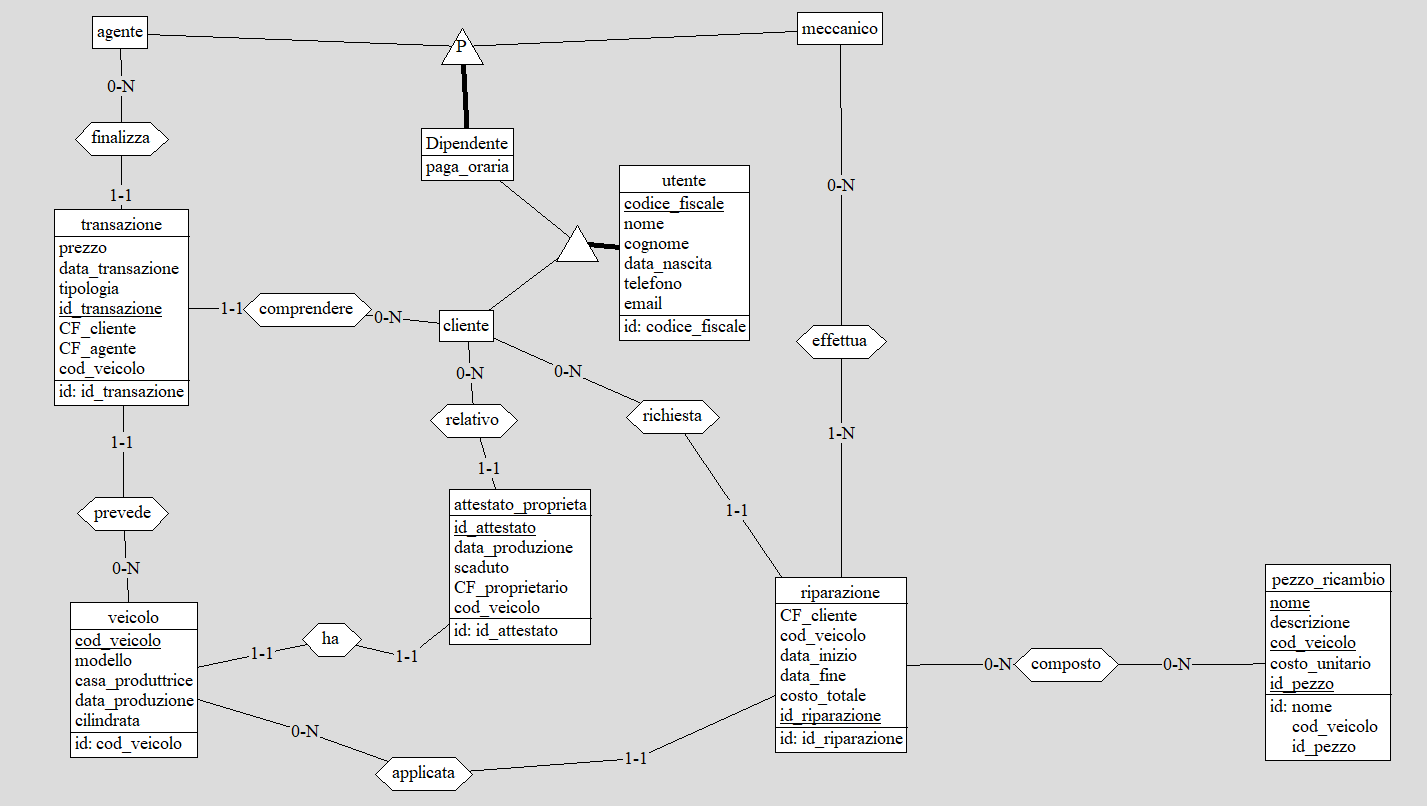
\includegraphics[scale=0.56]{img/schema_finale.png}
	\end{figure}

\chapter{Progettazione Logica}

\section{Stima Volume dati}
\begin{figure}[H]
	\fontsize{14pt}{12pt}\selectfont
	\advance\leftskip-15cm
	\centering
	\arrayrulecolor{BlueGreen}
	\begin{tabular}{l c c }
		\rowcolor{BlueGreen}
		\rule[-3mm]{0mm}{0.85cm}
		\textbf{Concetto} & \textbf{Costrutto} &\textbf{Volume} \\
		\hline\rule[-2mm]{0mm}{0.75cm}
		Utente & E & 3050\\
		\hline\rule[-2mm]{0mm}{0.75cm}
		Cliente & E & 3000 \\
		\hline\rule[-2mm]{0mm}{0.75cm}
		Dipendente & E & 50\\
		\hline\rule[-2mm]{0mm}{0.75cm}
		Agente & E & 20\\
		\hline\rule[-2mm]{0mm}{0.75cm}
		Meccanico & E & 30\\
		\hline\rule[-2mm]{0mm}{0.75cm}
		Possesso & R & 6000 \\
		\hline\rule[-2mm]{0mm}{0.75cm}
		Attestato & R & 6000\\
		\hline\rule[-2mm]{0mm}{0.75cm}
		Riguardo & R & 6000 \\
		\hline\rule[-2mm]{0mm}{0.75cm}
		Veicolo Nuovo & E & 120 \\
		\hline\rule[-2mm]{0mm}{0.75cm}
		Veicolo Usato & E & 6100 \\
		\hline\rule[-2mm]{0mm}{0.75cm}
		Coinvolgimento & R & 1000\\
		\hline\rule[-2mm]{0mm}{0.75cm}
		Transazione & R & 1000\\
		\hline\rule[-2mm]{0mm}{0.75cm}
		Transazione d'acquisto& R & 400\\
		\hline\rule[-2mm]{0mm}{0.75cm}
		Transazione di vendita& R & 600\\
		\hline\rule[-2mm]{0mm}{0.75cm}
		Perseguimento & R & 1000\\
		\hline\rule[-2mm]{0mm}{0.75cm}
		Esecuzione & R & 1000\\
		\hline\rule[-2mm]{0mm}{0.75cm}
		Lavorazione & R & 12000\\
		\hline\rule[-2mm]{0mm}{0.75cm}
		Riparazione & E & 12000\\
		\hline\rule[-2mm]{0mm}{0.75cm}
		Richiesta & R & 12000\\
		\hline\rule[-2mm]{0mm}{0.75cm}
		Sottoposizione & R & 12000\\
		\hline\rule[-2mm]{0mm}{0.75cm}
		Utilizzo & R & 15000\\
		\hline\rule[-2mm]{0mm}{0.75cm}
		Pezzo di ricambio & E &  9000\\
		\hline
	\end{tabular}
\end{figure}

\section{Descrizione operazioni principali e stima frequenza}
\begin{figure}[H]
	\fontsize{14pt}{12pt}\selectfont
	\advance\leftskip-15cm
	\centering
	\arrayrulecolor{BlueGreen}
	\begin{tabular}{c c c }
		\rowcolor{BlueGreen}
		\rule[-6mm]{0mm}{1.5cm}
		\textbf{Codice} & \textbf{Operazione} &\textbf{Frequenza} \\
		\hline\rule[-5mm]{0mm}{1.4cm}
		1 & Inserimento cliente & 8 al giorno \\
		\hline\rule[-5mm]{0mm}{1.4cm}
		2 & Inserimento veicolo usato & 10 al giorno \\
		\hline\rule[-5mm]{0mm}{1.4cm}
		3 & Inserimento riparazione & 18 al giorno \\
		\hline\rule[-5mm]{0mm}{1.4cm}
		4 & Vendita veicolo nuovo & 3 a settimana \\
		\hline\rule[-5mm]{0mm}{1.4cm}
		5 & Acquisto veicolo usato & 8 a settimana \\
		\hline\rule[-5mm]{0mm}{1.4cm}
		6 & Visualizza elenco clienti & 25 al giorno \\
		\hline\rule[-5mm]{0mm}{1.4cm}
		7 & Visualizza elenco veicoli nuovi & 10 al giorno \\
		\hline\rule[-5mm]{0mm}{1.4cm}
		8 & Visualizza elenco veicoli dei clienti & 28 al giorno \\
		\hline\rule[-5mm]{0mm}{1.4cm}
		9 & \quantities{Visualizza elenco veicoli\\usati in vendita} & 12 al giorno  \\
		\hline\rule[-5mm]{0mm}{1.4cm}
		10 & \quantities{Visualizza le case produttrici\\più carenti dell'anno} & 1 all'anno  \\
		\hline\rule[-5mm]{0mm}{1.4cm}
		11 & \quantities{Visualizza i 5 meccanici\\più laboriosi} & 1 al giorno \\
		\hline\rule[-5mm]{0mm}{1.4cm}
		12 & Visualizza l'agente del mese & 1 al mese \\
		\hline\rule[-5mm]{0mm}{1.4cm}
		13 & Aggiorna attributo e-mail & 5 a settimana \\
		\hline\rule[-5mm]{0mm}{1.4cm}
		14 & \quantities{Aggiorna attributo km percorsi\\in veicoli usati} & 1 alla settimana \\
		\hline
	\end{tabular}
\end{figure}
\newpage
\section{Schemi di navigazione e tabelle accessi}
\subsection*{Operazione 1: Inserimento cliente}
\begin{figure}[ht]
	\centering
	\arrayrulecolor{BlueGreen}
	\begin{tabular}{L{3cm}C{2cm}C{4.5cm}C{2cm}}
		\rowcolor{BlueGreen}\rule[-1.5mm]{0mm}{0.60cm}{}
		\textbf{Concetto} & \textbf{Costrutto} &\textbf{Accessi} & \textbf{Tipo} \\	
		\hline\rule[-2mm]{0mm}{0.65cm}{}
		Cliente & E & 1 & S \\
	\end{tabular}
	
	\begin{tabular}{C{13.9cm}}
		\rule[-3mm]{0mm}{0.85cm}{}	
		\cellcolor{BlueGreen} \textbf{\underline{Totale:} 1 S $\to$ 2 x 8 = 16 accessi al giorno}
	\end{tabular}
\end{figure}

\subsection*{Operazione 2: Inserimento veicolo usato}
\begin{figure}[ht]
	\centering
	\arrayrulecolor{BlueGreen}
	\begin{tabular}{L{3cm}C{2cm}C{4.5cm}C{2cm}}
		\rowcolor{BlueGreen}\rule[-2mm]{0mm}{0.6cm}{}
		\textbf{Concetto} & \textbf{Costrutto} &\textbf{Accessi} & \textbf{Tipo} \\
		\hline\rule[-2mm]{0mm}{0.65cm}{}
		Cliente & E & 3 000 & L \\
		\hline\rule[-2mm]{0mm}{0.65cm}{}
		Veicolo Usato & E & 1 & S \\
		\hline\rule[-2mm]{0mm}{0.65cm}{}
		Veicolo Usato & E & 1 & L \\
		\hline\rule[-2mm]{0mm}{0.65cm}{}
		Attestato & R & 1 & L \\
	\end{tabular}
	
	\begin{tabular}{C{13.9cm}}
		\rule[-3mm]{0mm}{0.85cm}{}	
		\cellcolor{BlueGreen} \textbf{\underline{Totale:} 1 S + 3 002 L $\to$ 3 004 x 10 = 30 040 accessi al giorno}
	\end{tabular}
\end{figure}

\subsection*{Operazione 3: Inserimento riparazione}
\begin{figure}[ht]
	\centering
	\arrayrulecolor{BlueGreen}
	\begin{tabular}{L{3.5cm}C{2cm}C{4.5cm}C{2cm}}
		\rowcolor{BlueGreen}\rule[-2mm]{0mm}{0.6cm}{}
		\textbf{Concetto} & \textbf{Costrutto} &\textbf{Accessi} & \textbf{Tipo} \\
		\hline\rule[-2mm]{0mm}{0.65cm}{}
		Cliente & E & 3 000 & L \\
		\hline\rule[-2mm]{0mm}{0.65cm}{}
		Cliente & E & 1 & L \\
		\hline\rule[-2mm]{0mm}{0.65cm}{}
		Veicolo Usato & E & 6 000 / 3 000 = 2 & L \\
		\hline\rule[-2mm]{0mm}{0.65cm}{}
		Veicolo Usato & E & 1 & L \\
		\hline\rule[-2mm]{0mm}{0.65cm}{}
		Meccanico & E & 30 & L \\
		\hline\rule[-2mm]{0mm}{0.65cm}{}
		Pezzo di ricambio & E & 9 000 / 6 000 = 1,5 & L \\
		\hline\rule[-2mm]{0mm}{0.65cm}{}
		Riparazione & E & 1 & S \\
		\hline\rule[-2mm]{0mm}{0.65cm}{}
		Riparazione & E & 1 & L \\
		\hline\rule[-2mm]{0mm}{0.65cm}{}
		Lavorazione & R & 1 & S \\
		\hline\rule[-2mm]{0mm}{0.65cm}{}
		Utilizzo & R & 1 & S \\
	\end{tabular}
	
	\begin{tabular}{C{13.9cm}}
		\rule[-3mm]{0mm}{0.85cm}{}	
		\cellcolor{BlueGreen} \textbf{\underline{Totale:} 3 S +  3 035,5 L $\to$ 3 041,5 x 18 = 54 747 accessi al giorno}
	\end{tabular}
\end{figure}

\newpage
\subsection*{Operazione 4: Vendita veicolo nuovo}
\begin{figure}[ht]
	\centering
	\arrayrulecolor{BlueGreen}
	\begin{tabular}{L{4.2cm}C{2cm}C{4.5cm}C{2cm}}
		\rowcolor{BlueGreen}\rule[-2mm]{0mm}{0.6cm}{}
		\textbf{Concetto} & \textbf{Costrutto} &\textbf{Accessi} & \textbf{Tipo} \\
		\hline\rule[-2mm]{0mm}{0.65cm}{}
		Cliente & E & 3 000 & L \\
		\hline\rule[-2mm]{0mm}{0.65cm}{}
		Agente & E & 20 & L \\
		\hline\rule[-2mm]{0mm}{0.65cm}{}
		Cliente & E & 1 & L \\
		\hline\rule[-2mm]{0mm}{0.65cm}{}
		Agente & E & 1 & L \\
		\hline\rule[-2mm]{0mm}{0.65cm}{}
		Veicolo Nuovo & E & 120 & L \\
		\hline\rule[-2mm]{0mm}{0.65cm}{}
		Veicolo Nuovo & E & 1 & L \\
		\hline\rule[-2mm]{0mm}{0.65cm}{}
		Veicolo Nuovo & E & 1 & S \\
		\hline\rule[-2mm]{0mm}{0.65cm}{}
		Veicolo Usato & E & 1 & S \\
		\hline\rule[-2mm]{0mm}{0.65cm}{}
		Attestato & R & 1 & S \\
		\hline\rule[-2mm]{0mm}{0.65cm}{}
		Transazione di vendita& R & 1 & S \\
	\end{tabular}
	
	\begin{tabular}{C{13.9cm}}
		\rule[-3mm]{0mm}{0.85cm}{}	
		\cellcolor{BlueGreen} \textbf{\underline{Totale:} 4 S +  3 143 L $\to$ 3 151 x 3 = 9 453 accessi a settimana}
	\end{tabular}
\end{figure}

\subsection*{Operazione 5: Acquisto veicolo usato}
\begin{figure}[ht]
	\centering
	\arrayrulecolor{BlueGreen}
	\begin{tabular}{L{4.5cm}C{2cm}C{4.5cm}C{2cm}}
		\rowcolor{BlueGreen}\rule[-2mm]{0mm}{0.6cm}{}
		\textbf{Concetto} & \textbf{Costrutto} &\textbf{Accessi} & \textbf{Tipo} \\
		\hline\rule[-2mm]{0mm}{0.65cm}{}
		Cliente & E & 3 000 & L \\
		\hline\rule[-2mm]{0mm}{0.65cm}{}
		Agente & E & 20 & L \\
		\hline\rule[-2mm]{0mm}{0.65cm}{}
		Cliente & E & 1 & L \\
		\hline\rule[-2mm]{0mm}{0.65cm}{}
		Agente & E & 1 & L \\
		\hline\rule[-2mm]{0mm}{0.65cm}{}
		Veicolo Usato & E & 6 000 / 3 000 = 2 & L \\
		\hline\rule[-2mm]{0mm}{0.65cm}{}
		Attestato & R & 1 & S \\
		\hline\rule[-2mm]{0mm}{0.65cm}{}
		Transazione d'acquisto& R & 1 & S \\
	\end{tabular}
	
	\begin{tabular}{C{13.9cm}}
		\rule[-3mm]{0mm}{0.85cm}{}	
		\cellcolor{BlueGreen} \textbf{\underline{Totale:} 2 S +  3 024 L $\to$ 3 028 x 8 = 24 224 accessi a settimana}
	\end{tabular}
\end{figure}

\section{Raffinamento schema}
...eliminazione di identificatori esterni, attributi composti e gerarchie, scelta delle chiavi

\section{Analisi ridondanze}

\section{Traduzione di entità e associazioni in relazioni}

\section{Schema relazionale finale}

\section{Traduzione delle operazioni in query SQL}

\chapter{Progettazione Applicazione}

\section{Descrizione applicazione}
Per la gestione dell'officina è stata realizzata un'applicazione web in php che usa MySQLi, per  
%
comunicare con il DBMS MySQL, e javascript per funzionalità dinamiche di visualizzazione del sito.

Come prima pagina troviamo l'elenco dei collegamenti per le quattro macro categorie in cui si può dividere la base 
%
di dati, con il nome della categoria e sotto una breve descrizione del contenuto. 
%
Infondo a questa, ma anche a tutte le altre pagine, è presente uno spazio contenente i contatti dell'officina.

Andiamo ad analizzare una ad una ogni pagina e le relative sotto categorie.

\subsection*{Pagina Clienti}
In questa pagina ci viene mostrato il form attraverso il quale è possibile inserire un nuovo cliente, specificandone
%
tutti gli attributi, la mail è opzionale, che verranno controllati opportunamente prima di essere inseriti.

Sotto il form d'inserimento troviamo una tabella che ha per righe i clienti registrati e come colonne i vari attributi	
%
inseriti, in fondo alla tabella è possibile inoltre, per ogni singolo cliente, aggiornare telefono, mail o entrambi.

\subsection*{Pagina Agenti}
In questa pagina abbiamo la possibilità di scegliere tra due sezioni:

\subsubsection*{Pagina Gestione Agenti}
In questa pagina è possibile inserire e visualizzare gli agenti esattamente come per la pagina dei clienti, con 
%
l'aggiunta dell'attributo paga oraria all'inserimento e dunque anche della sua presenza nella tabella degli attributi.
%
Questo parametro, inoltre, può essere aggiornato proprio come mail e telefono.

\subsubsection*{Pagina Transazioni}
Qua è possibile registrare una transazione specificando per primi agente e cliente coinvolti, poi verrà mostrata la lista
%
dei veicoli da consultare in base alla scelta della tipologia di auto: nuova o usata e il tipo di transazione: acquisto o vendita.

Nella parte inferiore invece è possibile visualizzare tutti i passaggi effettuati con la relativa data.

\subsection*{Pagina Meccanici}
In questa pagina abbiamo la possibilità di scegliere tra tre sezioni:

\subsubsection*{Pagina Gestione Meccanici}
In questa pagina è possibile inserire e visualizzare gli agenti esattamente come per la pagina degli agenti.

\subsubsection*{Pagina Riparazioni}
Qui è possibile registrare una riparazione specificando in ordine: prima il cliente, poi l'auto in oggetto, tra quelle 
%
di proprietà del cliente, infine saranno selezionabili i vari meccanici coinvolti, pezzi utilizzati e gli altri attributi.

\subsubsection*{Pagina Pezzi di ricambio}
In questa pagina si inseriscono i pezzi di ricambio e si può vedere la lista di quelli già presenti.

\subsection*{Pagina Veicoli}
In questa pagina abbiamo la possibilità di scegliere tra due sezioni:

\subsubsection*{Pagina Gestione Veicoli Nuovi}
In questa sezione si registrano e visualizzano solo i veicoli nuovi da registrare in officina.

\subsubsection*{Pagina Gestione Veicoli Usati}
In questa parte invece si possono inserire i veicoli usati, specificandone il cliente, e si possono inoltre 
%
consultare una tabella contente i veicoli appartenti ai vari clienti registrati e una tabella con i veicoli
%
usati di proprietà dell'officina. In fondo ad ogni riga di quest'ultima tabella, c'è un link che porta alla pagina
% 
delle transazioni dove è possibile acquistare l'auto.

DA INSERIRE: Screenshot interfaccia utente

\end{document}
